\chapter{Introduzione}
\section{Sistema Operativo}
\begin{defn}[Sistema Operatvio]
  Un sistema operatvio è un \textbf{software} che agisce come intermediario fra l'hardware e l'utente.
\end{defn}
Ha diversi obiettivi:
\begin{itemize}
  \item Eseguire programmi dell'utente.
  \item Far diventare l'uso del dispositivo conveniente.
  \item Usare l'hardware del computer in modo efficiente.
\end{itemize}
Per capire bene cosa fa un sistema opertivo è utili dividere la struttura di un computer in quattro parti principali:
\begin{enumerate}
  \item \textbf{Hardware:} provvede le risorse basi, come la cpu, la memoria centrale e i dispositivi di I/O. 
  \item \textbf{Sistema operativo:} controlla e gestisce l'hardware per applicazioni e utenti.
  \item \textbf{Programmi applicativi:} decide come le risorse hardware devono essere divise fra i vari programmi.
  \item \textbf{Utenti:} agenti esterni che interagiscono con il computer.
\end{enumerate}

\begin{figure}[!htb]
    \centering
    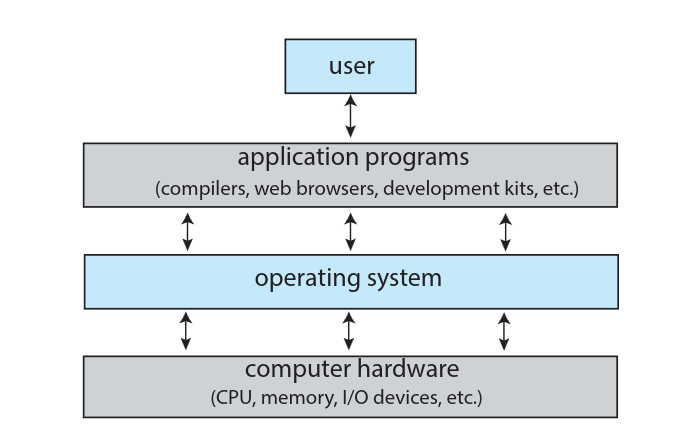
\includegraphics[width=0.5\linewidth]{Images/intro/os.png}
    \caption{Architettura del sistema di un computer.}
\end{figure}

Dal punto di vista di un utente, deve essere facile usare applicazioni e avere buone prestazioni. \\
Dal punto di vista del computer, però, tutti gli utente devono essere soddisfatti, quindi il sistema operativo deve essere un \textbf{allocatore di risorse} e un \textbf{gestore di programmi}.

\newpage
\section{Organizzazione del Sistema di un Computer}
Un computer moderno \textbf{general-purpose} consiste in una o più CPU e un numero di dispositivi che sono collegati tramite un \textbf{bus} comune che da accesso alla memoria condivisa e agli altri componenti.

\begin{figure}[!htb]
    \centering
    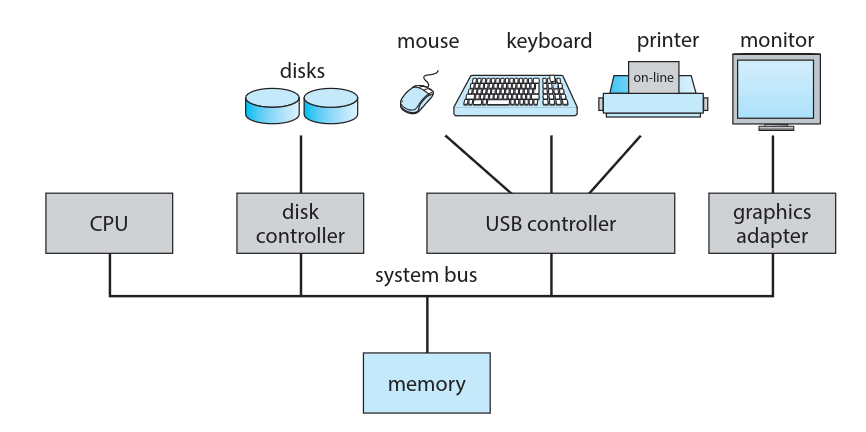
\includegraphics[width=0.6\linewidth]{Images/intro/org.png}
    \caption{Organizzazione del sistema di un computer.}
\end{figure}

Ogni dispositivo ha un controller, che si occupa di gestire i dati fra il suo buffer interno e altri componenti. \\
I sistemi operatvi per interagire in modo uniforme con i controller, usano dei \textbf{driver}. 
Dato che la CPU e i controller possono agire in parallelo, competendo per cicli di memeoria, bisogna trovare un modo ordinato per l'accesso alla memoria condivisa.

\subsection{Interrupt}
\begin{ex}[Operazione di I/O]
  Per un'operazione di I/O si succedono diverse azioni:
  \begin{itemize}
    \item Il driver carica correttamente i registri del controller.
    \item Il controller guarda i regsitri per capire che operazione fare.
    \item Il controller carica i dati da un dispositivo al suo buffer locale.
    \item Il controller informa il driver di aver finito l'operazione.
  \end{itemize}
  Per ultimo, il driver da il controllo al sistema operativo, passando i dati letti o un puntatore a questi.
\end{ex}
Il controller per avvisare il driver di aver finito la sua operazione, usa una \textbf{interrupt}.

\begin{figure}[!htb]
    \centering
    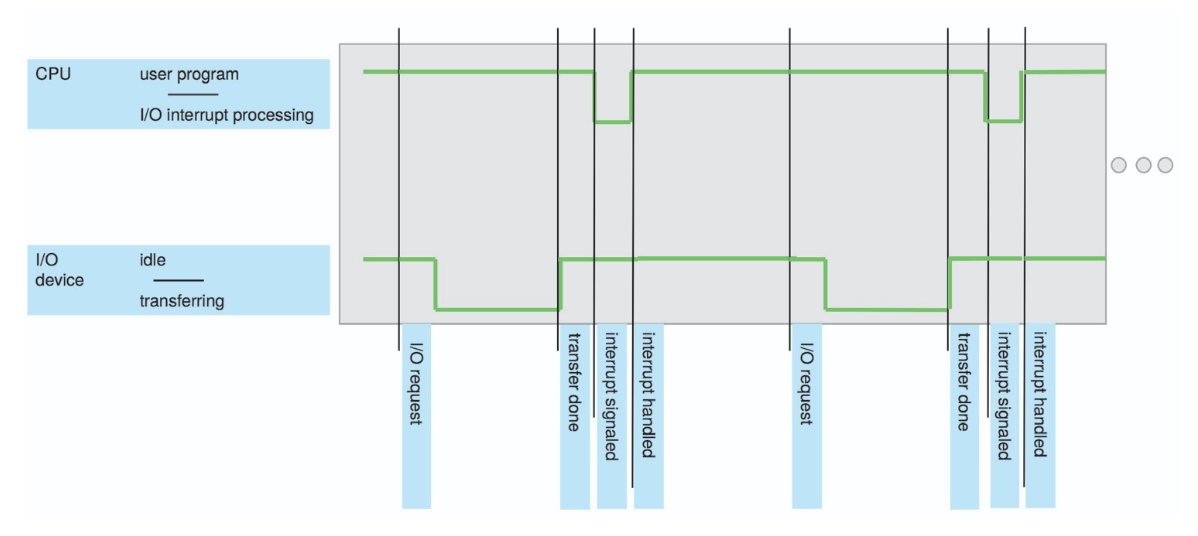
\includegraphics[width=0.8\linewidth]{Images/intro/interrupt.png}
    \caption{Timeline di una interrupt.}
\end{figure}

Quando la CPU riceve una interrupt, ferma immediatamente quello che sta facendo e trasferisce l'esecuzione alla service routine corretta, fino a che non è stata completata. 
Una volta finita, la CPU ricomincia da dove aveva interrotto, inserendo nel \textbf{program counter} l'indirizzo corretto. 
\begin{note}[NOTA BENE]
Questa metodologia richiede, però, di dover salvare lo stato delle informazioni della CPU, dato che le service routine degli interrupt potrebbero modificare i registri.
\end{note}
Le interrupt, dato che sono molto frequenti, devono essere gestite velocemente. Per questo, si può usare una tabella, salvata nella parte basse della memoria,
che contiene tutti gli indirizzi delle service routine degli interrupt, garantendo la velocità necessaria. Questo array (o \textbf{vettore degli interrupt}) di indirizzi, 
ha come indici dei numeri univoci che specificano la routine corretta per il tipo di interrupt.

\begin{figure}[!htb]
    \centering
    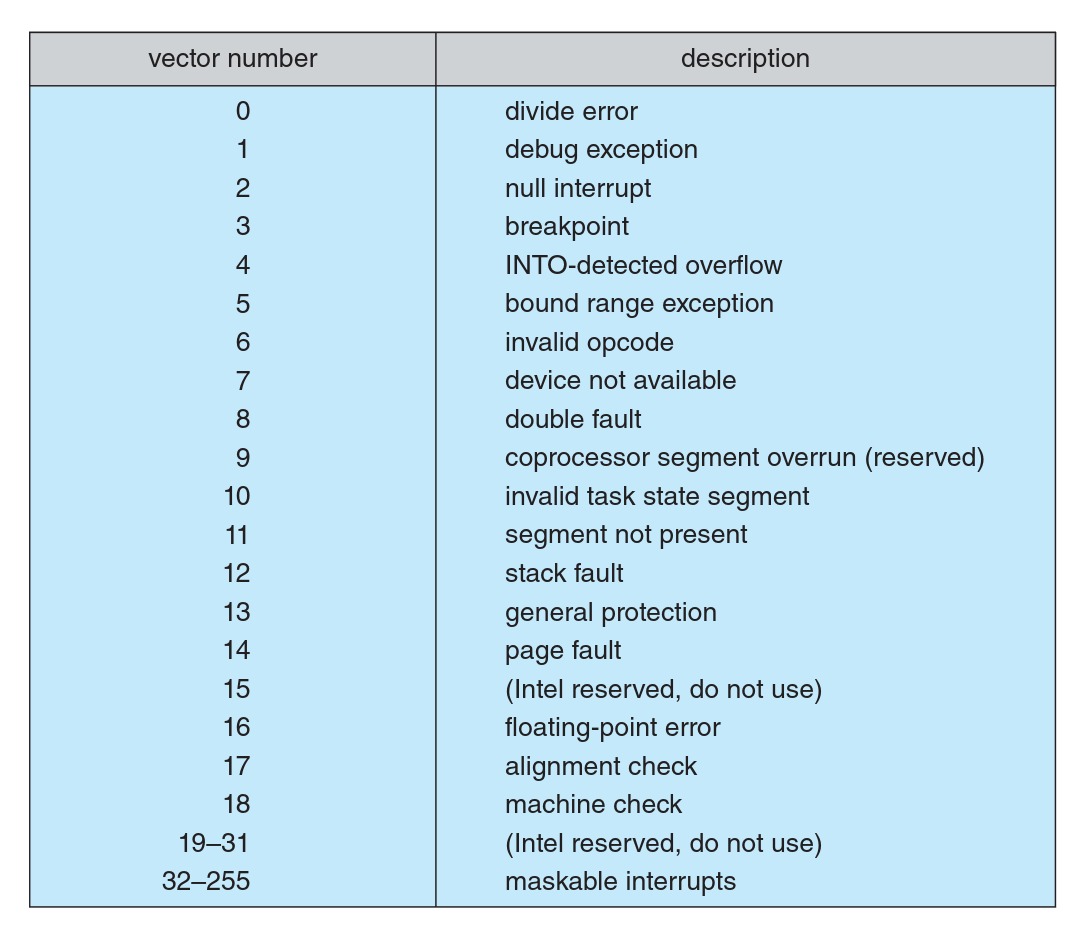
\includegraphics[width=0.6\linewidth]{Images/intro/vector.png}
    \caption{Tabella degli indici di un vettore di interrupt.}
\end{figure}

\subsubsection{Implementazione}
L'hardware della CPU ha un cavo chiamato \textbf{interrupt-request line}, dove la CPU riceve i segnali dai controller. Una volta intercettato il numero dell'interruzione, tramite il vettore degli interrupt, 
viene chiamata l'\textbf{interrupt-handler routine} corretta. \\ 
In sistemi operativi moderni, il metodo deve essere più sofisticato:
\begin{itemize}
  \item È necessaria la possibilità di differire la gestione delle interruzioni durante l'esecuzione di elaborazioni critiche.
  \item È necessario un metodo efficiente per indirizzare l'esecuzione all'interrupt-handler corretto per un determinato dispositivo.
  \item Sono necessarie interruzioni multilivello, in modo che il sistema operativo possa distinguere tra interruzioni ad alta e bassa priorità e rispondere con il livello di urgenza adeguato.
\end{itemize}
Queste tre caratteristiche sono fornite dalla CPU e dall'\textbf{interrupt-controller hardware}. \\
\vspace*{0.01\textheight}
Per gestire la priorità tra interrupt, nelle CPU esistono due linee di richieste per le interruzioni:
\begin{enumerate}
  \item \textbf{Maskable:} può essere momentaneamente spenta dalla CPU, per dare priorità a istruzioni critiche. Questa linea è usata dai controller dei dispotivi.
  \item \textbf{Non-Maskable:} usata per interrupt che non possono essere ignorate, come errori di memoria non recuperabili.
\end{enumerate}

\subsection{Struttura della Memoria}
La memoria di un computer è organizzata in un gerarchia che tiene conto di tre valori:
\begin{enumerate}
  \item \textbf{Velocità}.
  \item \textbf{Capacità}.
  \item \textbf{Volatilità}.
\end{enumerate}

\begin{figure}[!htb]
    \centering
    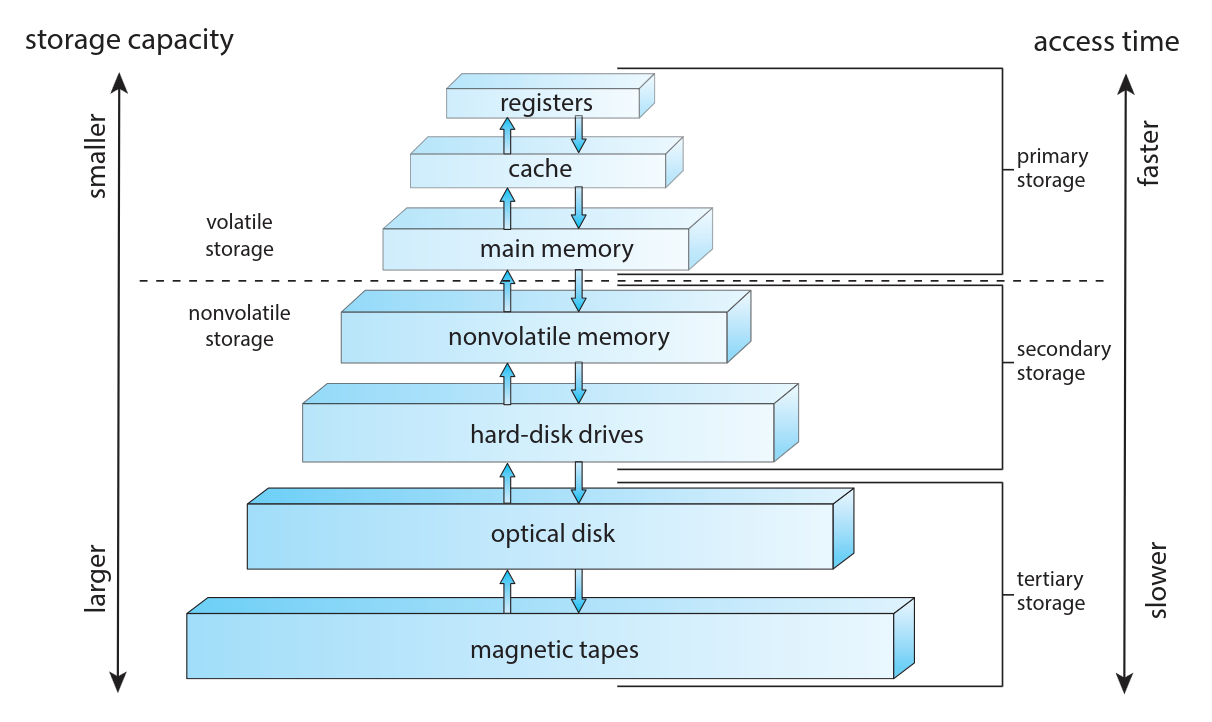
\includegraphics[width=0.6\linewidth]{Images/intro/memorie.png}
    \caption{Gerarchia delle memorie.}
\end{figure}

Per spostare grandi quantità di dati, la metodologia degli interrupt descritta prima potrebbe creare molto overhead, per questo viene usata la \textbf{DMA} (\textbf{Direct Memory Access}).
\begin{defn}[Direct Memory Access]
Dove aver sistemato buffer e puntatori, il controller del dispositivo sposta un grande blocco di dati dalla memoria al componente, o viceversa, senza l'intervento della CPU.
Questo genera una sola interrupt per blocco, a discapito delle numerose interrupt generate senza DMA.
\end{defn}

\section{Architetture dei Computer}
Possono esistere diverse architetture, basate sul numero di processori presenti all'interno del computer:
\begin{itemize}
  \item \textbf{Single-Processor:} se è presente un solo processore.
  \item \textbf{Multi-Processor:} attualmente comune come \textbf{Multi-Core}, se sono presenti più processori. Condividono la memoria centrale e i dispositivi di I/O.
  \item \textbf{Cluster:} si distinguono dai computer multi-processor, perchè sono sistemi autonomi che lavorano insieme. Ogni nodo è spesso un computer multi-core.
\end{itemize}

\begin{defn}[Alcune concetti di base]
\textbf{CPU:} hardware che esegue le istruzioni. \\
\textbf{Processor:} chip che contiene una o più CPU. \\
\textbf{Core:} unità basica della CPU.
\end{defn}

\section{Operazioni di un Sistema Operativo}
Per avviare il computer, è necessario un programma di iniziale: il \textbf{bootstrap}.
Serve a inizializzare tutte le risorse utili, come registri e i vari controller. 
In ultimo, deve localizzare il kernel del sistema operativo e caricarlo in memoria. \\ 
\vspace*{0.01\textheight}
Il sistema operativo, in assenza di azione da eseguire, aspetta degli eventi, come le interrupt a livello hardware o le \textbf{trap} (\textbf{exceptions}) a livello software.

\subsection{Multitasking e Multiprogramming}
L'obiettivio del sistema operativo è tenere la CPU occupata tutto il tempo e nel mentre garantire all'utente di utilizzare più programmi contemporaneamente. 
Tutto questo è fattibile grazie alla capacità di essere multiprogramming, potendo gestire più programmi in esecuzione o \textbf{processi}. \\ 
Invece, il multitasking, è la capacità di poter saltare da un processo all'altro velocemente, garantendo un tempo di risposta molto basso all'utente.

\subsection{Operazioni Dual-Mode}
\begin{note}[Problema]
Il sistema operativo e gli utenti risiedono sullo stesso hardware.
Si deve trovare una soluzione per evitare di eseguire codice malevolo che potrebbe alterare il funzionamento di altri programmi o del sistema stesso.
\end{note}
Come minimo, sono necessarie due modalità: \textbf{Kernel Mode} e \textbf{User Mode}. All'hardware è stato aggiunto un bit, chiamato \textbf{bit mode}, che permette di distinguere la modalità corrente: kernel (0) e user (1).

\begin{figure}[!htb]
    \centering
    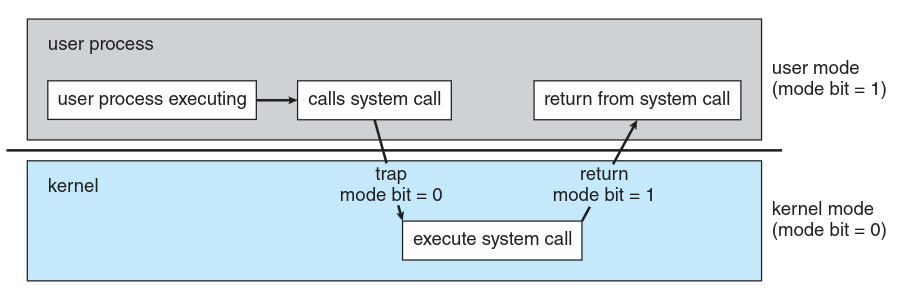
\includegraphics[width=0.8\linewidth]{Images/intro/bitmode.png}
    \caption{Operazione Dual-Mode.}
\end{figure}

Se si prova a eseguire una istruzione vietata in user mode, allora l'hardware lancerà una trap al sistema operativo, 
il quale tramite il vettore delle interrupt, prende il controllo e termina l'esecuzione del processo.

\subsection{Timer}
Bisogna assicurarsi che il sistema operativo mantenga sempre il controllo sulla CPU,
per evitare che programmi in esecuzione dell'utente si blocchino in un loop infinito, oppure che una system call fallita non ritorni il controllo al sistema operativo. \\ 
Una soluzione è usare un \textbf{timer}, che interrompe il computer dopo un certo periodo.
\vspace*{0.01\textheight}
Solitamente, viene implementato tramite un clock a frequenza fissa e un contatore. Ogni ciclo di clock, il contatore viene diminuito di una unità.

\begin{note}[Timer su Sistemi Linux]
Nei sistemi Linux, il parametro di configurazione del kernel \texttt{HZ} specifica la frequenza delle interrupt del timer. Per esempio, \texttt{HZ} $= 250$, significa 250 interruzioni al secondo o una ogni 4 millisecondi.
\end{note}

\section{Sicurezza e Protezione}
Nei sistemi operativi moderni, che supportano più utenti, i dati che vengono usati devono essere garantita solo al processo che ha ricevuto tutte le autorizzazioni.

\begin{defn}[Protezione]
Qualsiasi meccanismo per controllare l'accesso alle risorse di un computer da parte di utenti o processi. \\
Deve essere possibile avere un modo per specificare i controlli e controllare che vengano rispettati.
\end{defn}
Anche se è presente un alto grado di protezione, può rimanere comunque vulnerabile a fallimenti o accessi non autorizzati.
\begin{defn}[Sicurezza]
Difendere il sistema da attacchi interni ed esterni, come dos, worms, furti di dati e identità, ecc...
\end{defn}
I sistemi operativi per distinguere fra gli utenti, usa diversi identificativi:
\begin{itemize}
  \item \textbf{User ID:} nome e numero associato a ogni utente.
  \item \textbf{Group Identifier:} per definire un gruppo di utenti e associargli risorse e processi.
\end{itemize}
Per ottenere più permessi, è possibile fare \textbf{privilage escalation} per cambiare il proprio ID e avere più permessi.
